\begin{frame}[noframenumbering]
	\centering
	\huge Our Adaptive SPS \\ Predictive approach (PA-SPS)
\end{frame}


\begin{frame}{Predictive Approach : PA-SPS}
	\begin{block}{Proposal}
		\textbf{Estimate the number of active replicas} for operator according to the predicted input rate
	\end{block}
\end{frame}

\begin{frame}{Predictive Approach : PA-SPS}
	Predictor model is based in : 
	\begin{itemize}
		\item number of events received
		\item dependency among operators
		\item number of queued events
	\end{itemize}
\end{frame}

\begin{frame}{Predictive Approach : PA-SPS}
\begin{figure}
    \centering
    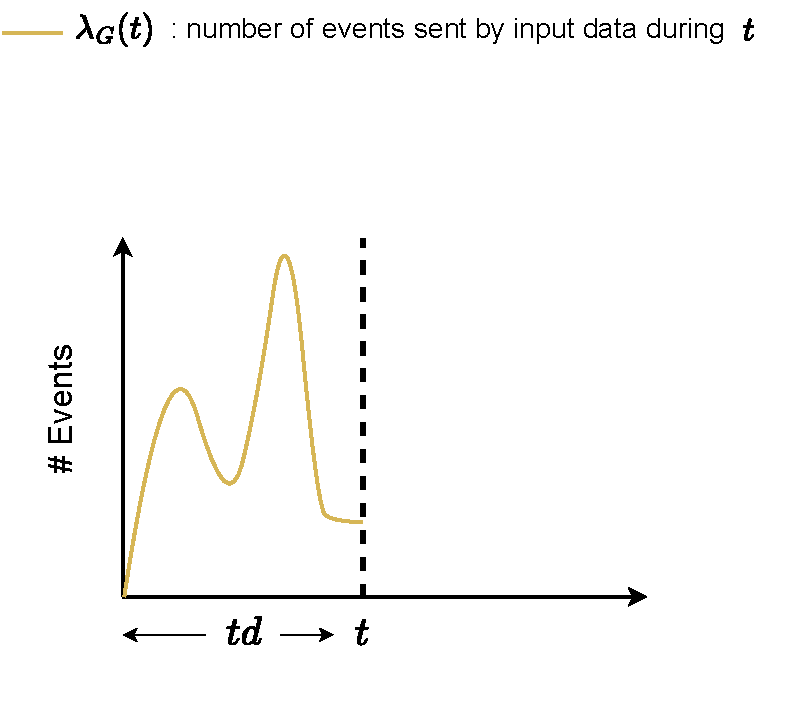
\includegraphics[scale=0.63]{images/concepts/predictive/PA-SPS-Prediction-1.pdf}
\end{figure}
\end{frame}

\begin{frame}{Predictive Approach : PA-SPS}
\begin{figure}
    \centering
    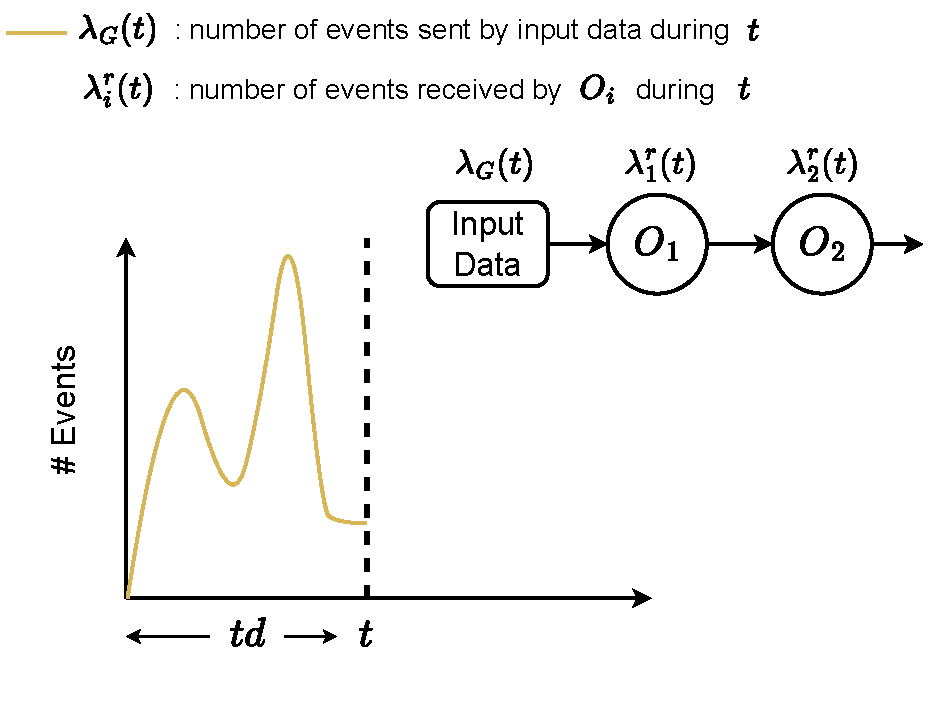
\includegraphics[scale=0.63]{images/concepts/predictive/PA-SPS-Prediction-2.pdf}
\end{figure}
\end{frame}

\begin{frame}{Predictive Approach : PA-SPS}
\begin{figure}
    \centering
    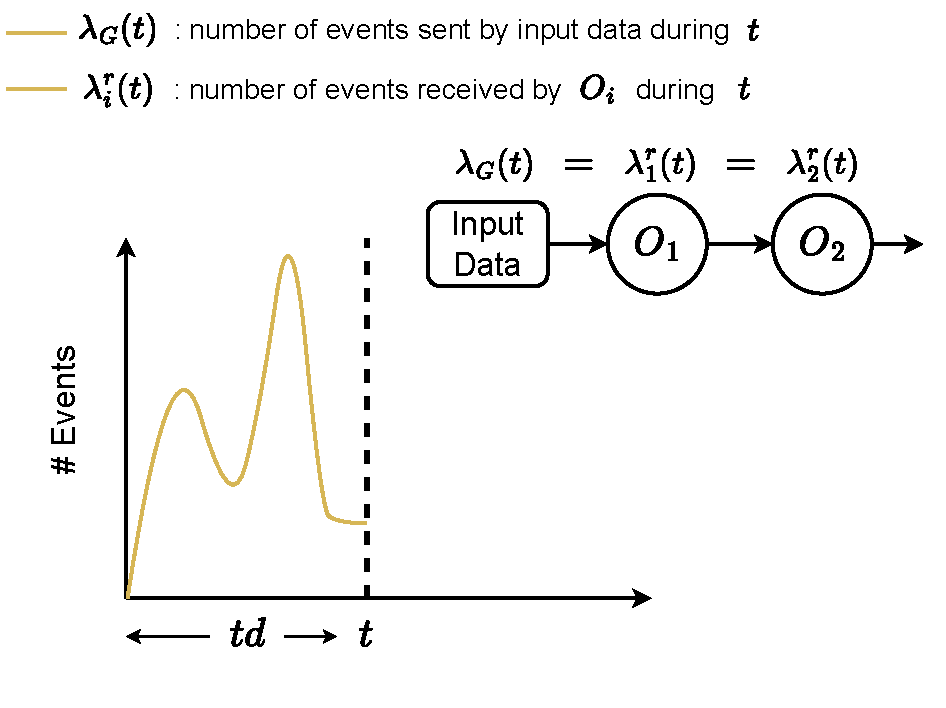
\includegraphics[scale=0.63]{images/concepts/predictive/PA-SPS-Prediction-3.pdf}
\end{figure}
\end{frame}

\begin{frame}{Predictive Approach : PA-SPS}
\begin{figure}
    \centering
    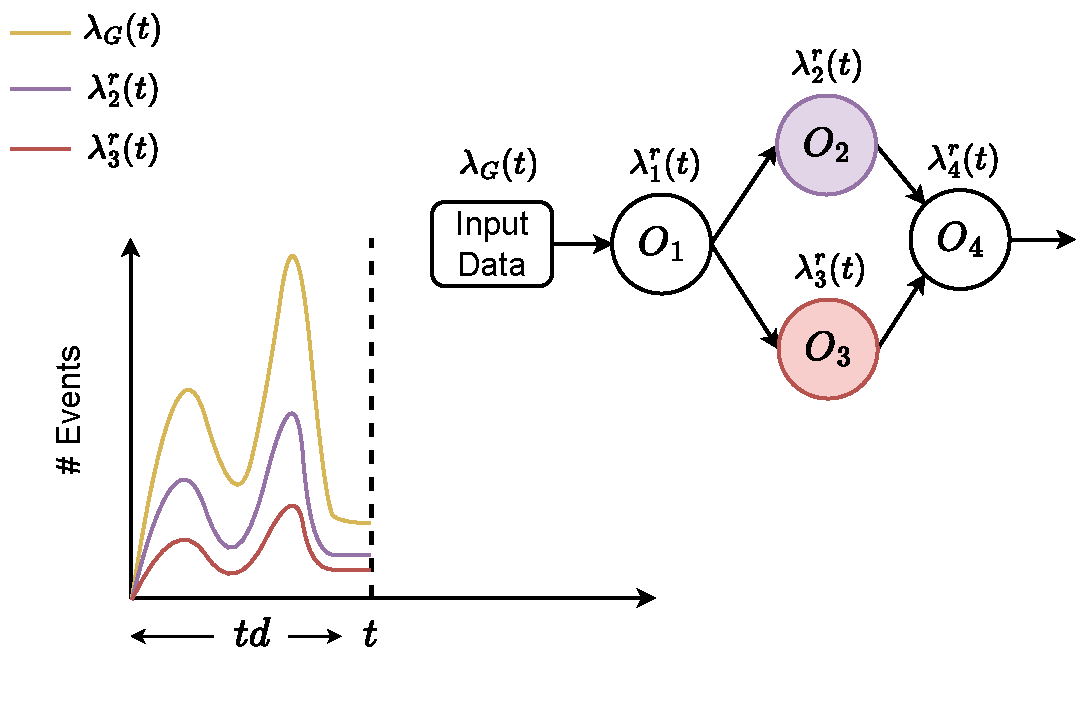
\includegraphics[scale=0.63]{images/concepts/predictive/PA-SPS-Prediction-4.pdf}
\end{figure}
\end{frame}

\begin{frame}{Predictive Approach : PA-SPS}
\vspace*{-0.5cm}
\begin{figure}
    \centering
    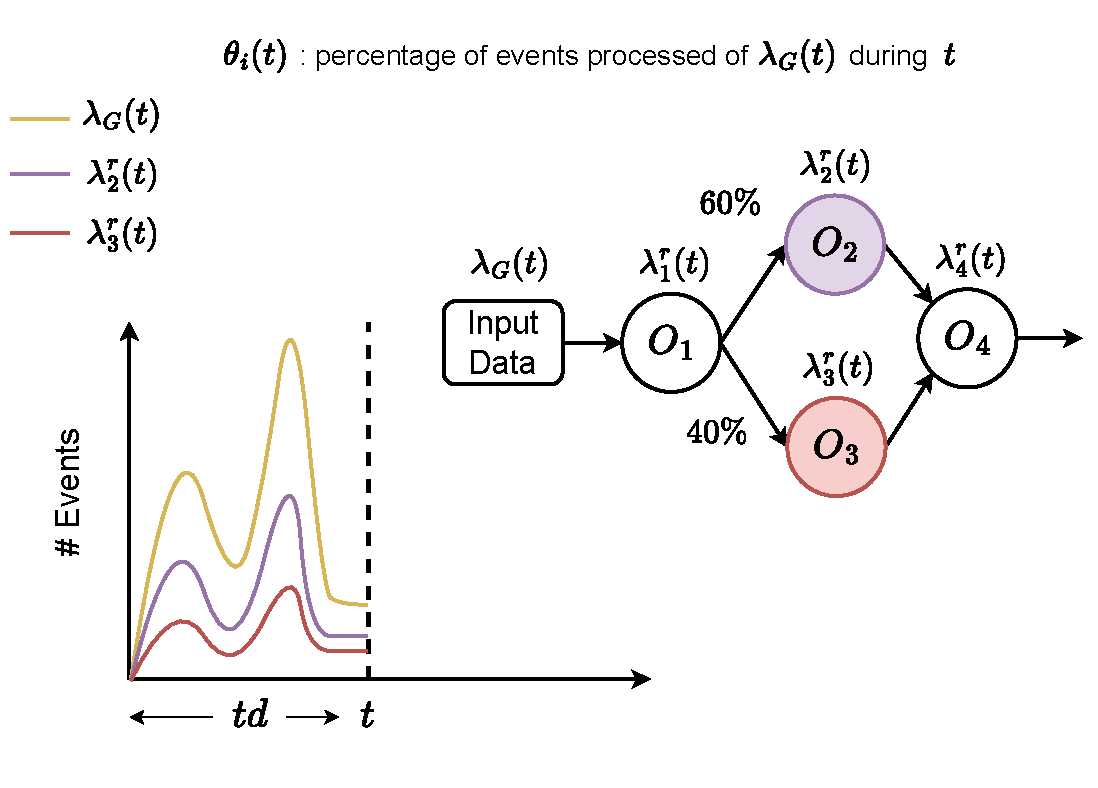
\includegraphics[scale=0.6]{images/concepts/predictive/PA-SPS-Prediction-5.pdf}
\end{figure}
\end{frame}

\begin{frame}{Predictive Approach : PA-SPS}
\begin{figure}
    \centering
    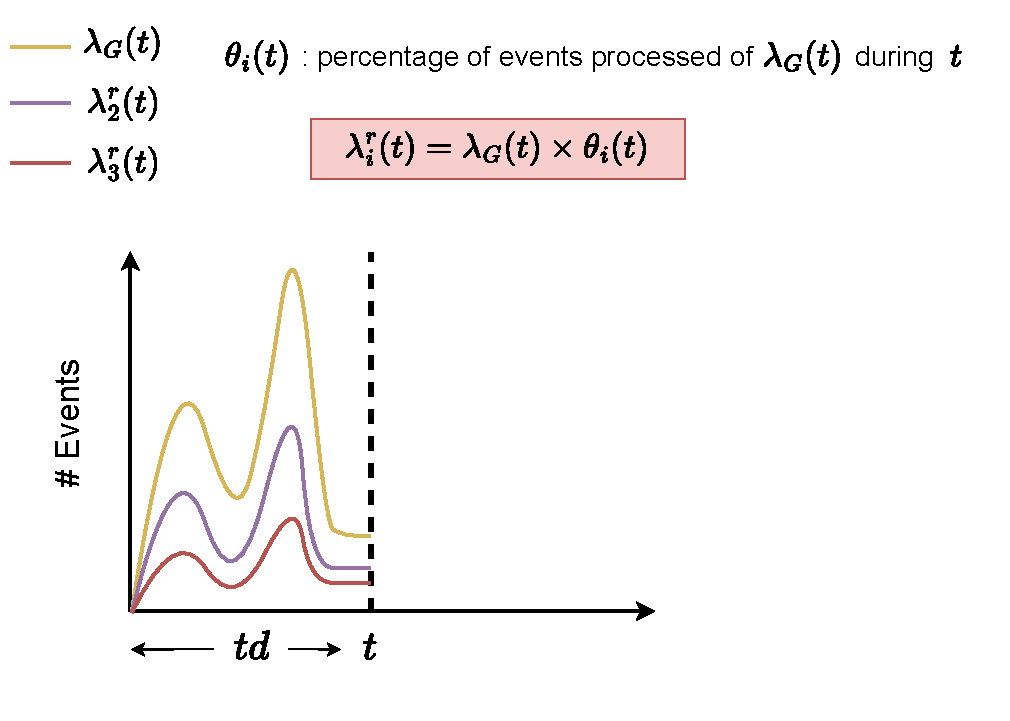
\includegraphics[scale=0.63]{images/concepts/predictive/PA-SPS-Prediction-6.pdf}
\end{figure}
\end{frame}

\begin{frame}{Predictive Approach : PA-SPS}
\begin{figure}
    \centering
    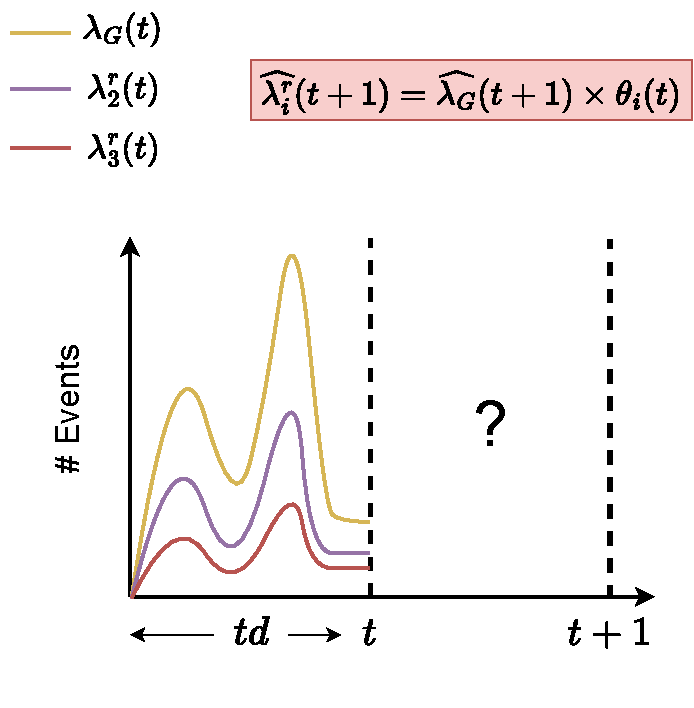
\includegraphics[scale=0.63]{images/concepts/predictive/PA-SPS-Prediction-7.pdf}
\end{figure}
\end{frame}

\begin{frame}{Predictive Approach : PA-SPS}
	\textbf{Predictive model} is used to predict the number of events sent by the input data during the next time interval\\
	\vspace*{0.25cm}
	Predictive models applied:
	\begin{itemize}
		\item Basic
		\item Linear regression
		\item Fast Fourier Transform
		\item Artificial Neural Network
		\item Random Forest
	\end{itemize}

\end{frame}

\begin{frame}{Predictive Approach : PA-SPS}
\begin{figure}
    \centering
    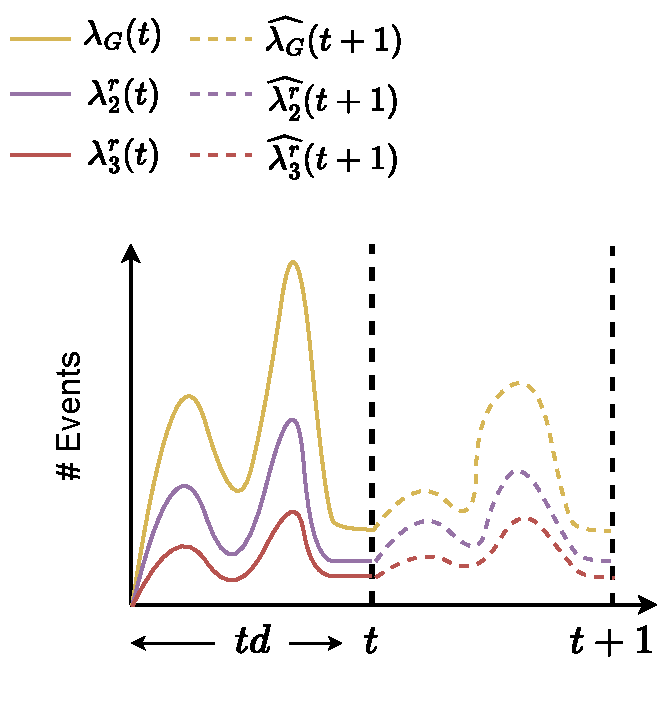
\includegraphics[scale=0.63]{images/concepts/predictive/PA-SPS-Prediction-8.pdf}
\end{figure}
\end{frame}

\begin{frame}{Predictive Approach : PA-SPS}
\begin{figure}
    \centering
    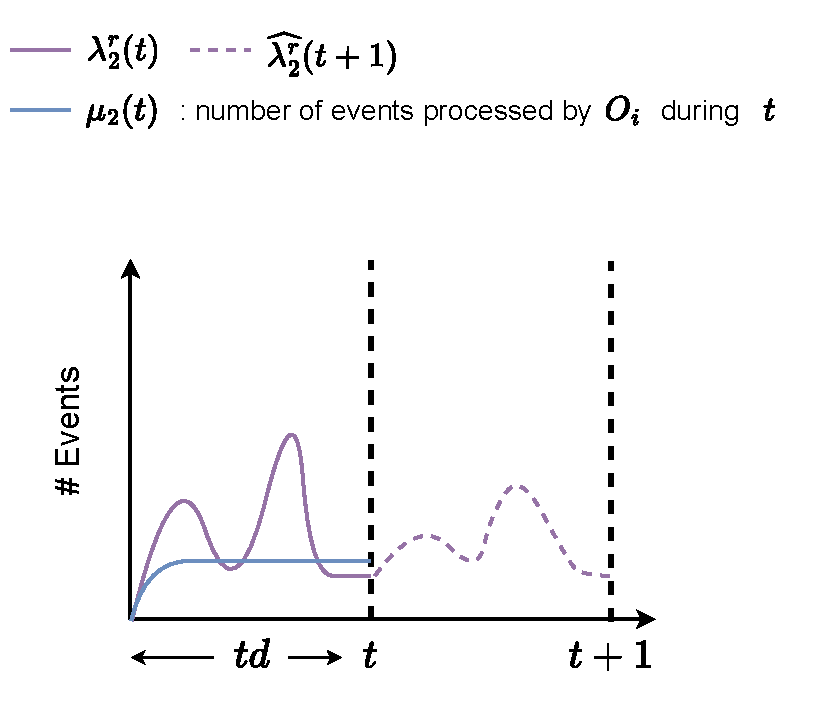
\includegraphics[scale=0.63]{images/concepts/predictive/PA-SPS-Prediction-9.pdf}
\end{figure}
\end{frame}

\begin{frame}{Predictive Approach : PA-SPS}
\begin{figure}
    \centering
    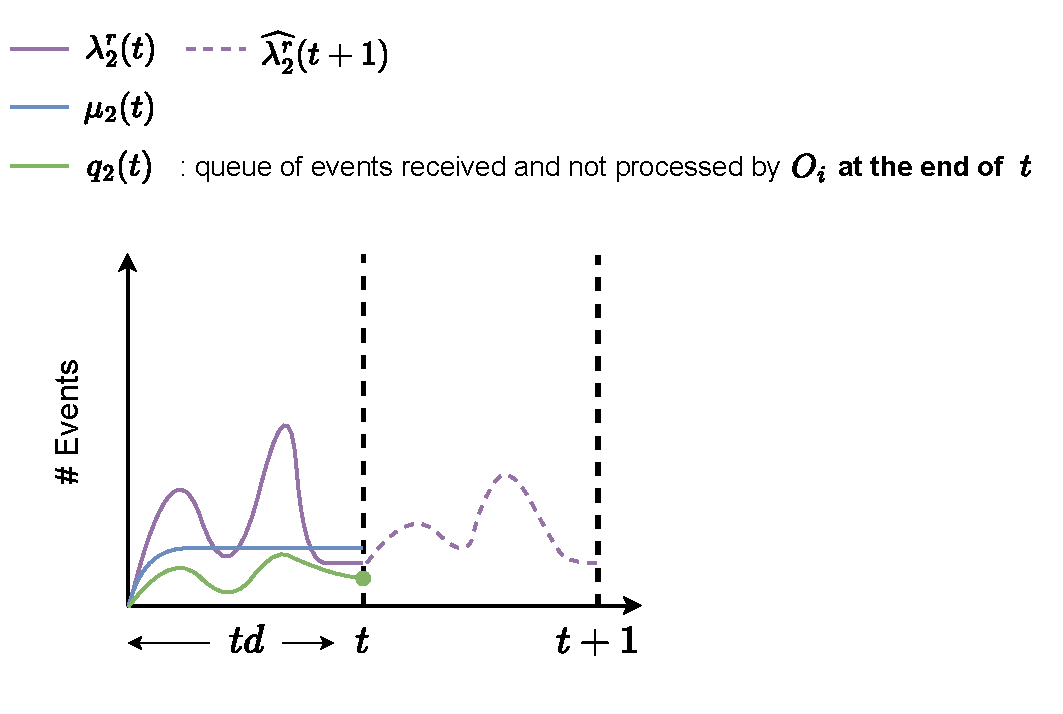
\includegraphics[scale=0.63]{images/concepts/predictive/PA-SPS-Prediction-10.pdf}
\end{figure}
\end{frame}

\begin{frame}{Predictive Approach : PA-SPS}
\begin{figure}
    \centering
    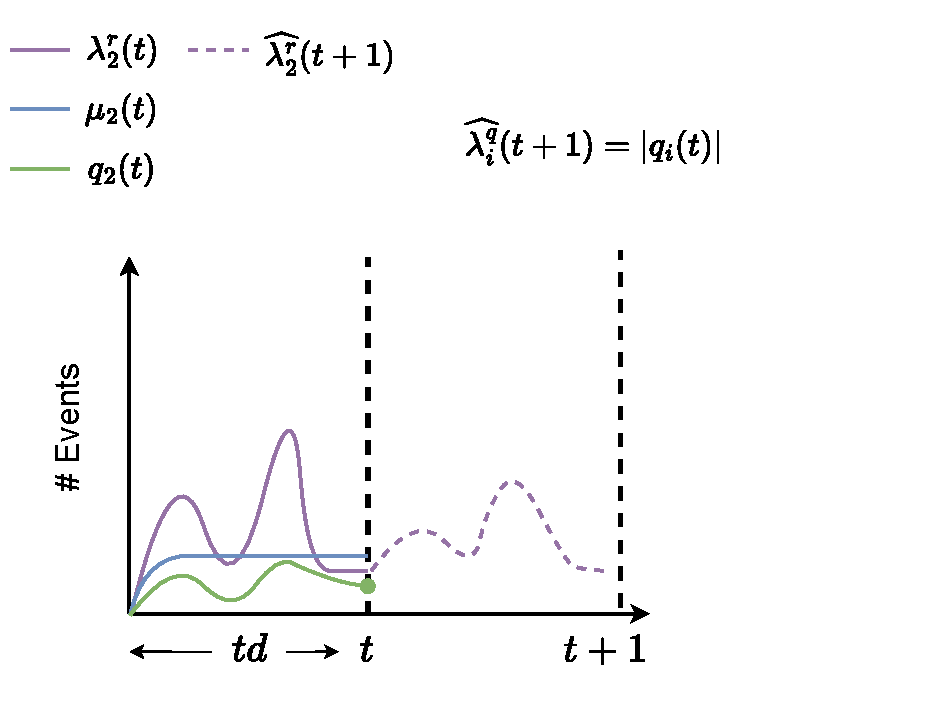
\includegraphics[scale=0.63]{images/concepts/predictive/PA-SPS-Prediction-10-2.pdf}
\end{figure}
\end{frame}

\begin{frame}{Predictive Approach : PA-SPS}
\begin{figure}
    \centering
    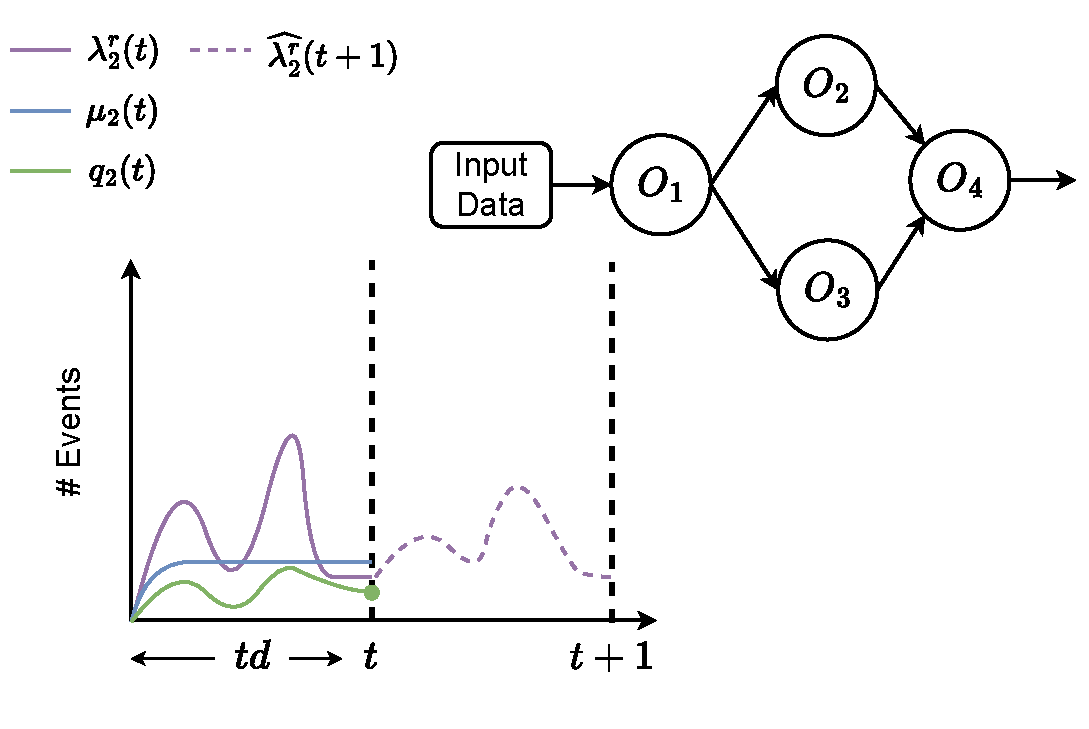
\includegraphics[scale=0.63]{images/concepts/predictive/PA-SPS-Prediction-11.pdf}
\end{figure}
\end{frame}

\begin{frame}{Predictive Approach : PA-SPS}
\begin{figure}
    \centering
    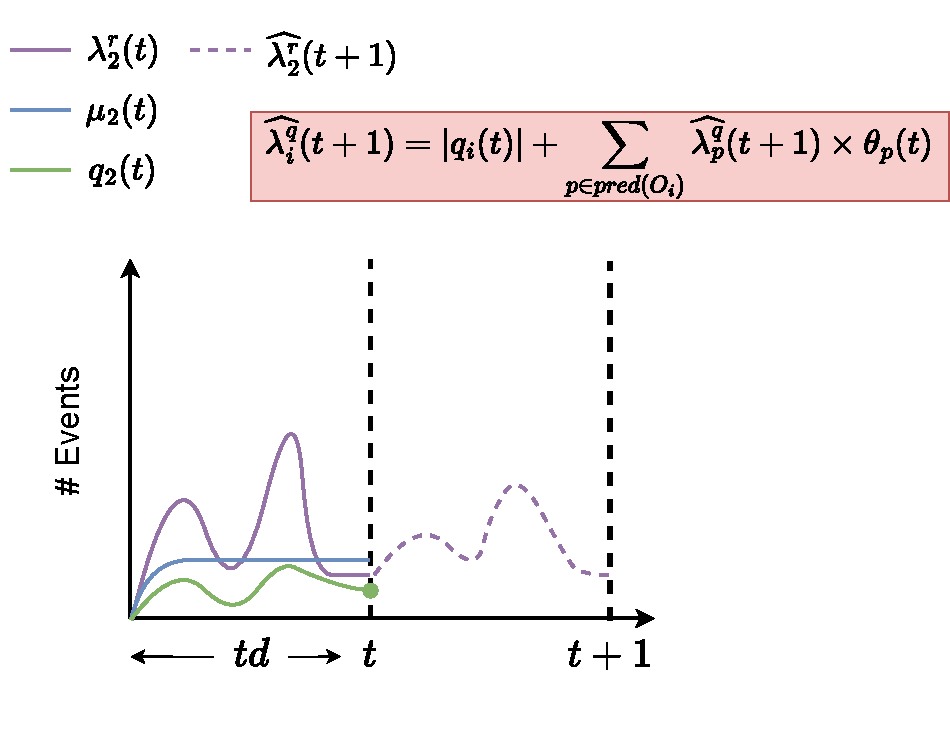
\includegraphics[scale=0.63]{images/concepts/predictive/PA-SPS-Prediction-12.pdf}
\end{figure}
\end{frame}

\begin{frame}{Predictive Approach : PA-SPS}
\begin{figure}
    \centering
    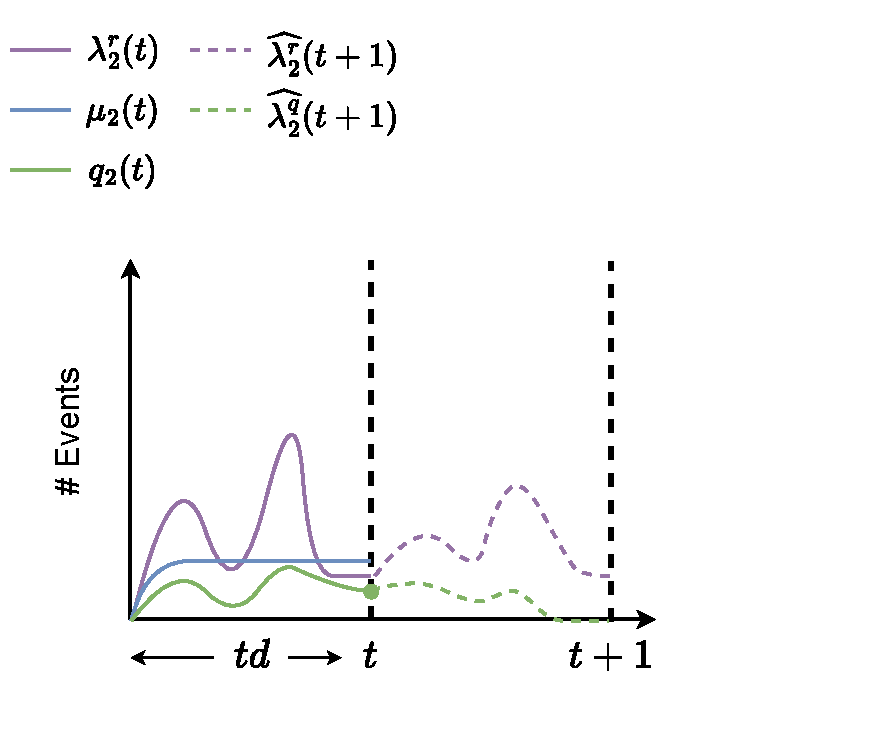
\includegraphics[scale=0.63]{images/concepts/predictive/PA-SPS-Prediction-13.pdf}
\end{figure}
\end{frame}

\begin{frame}{Predictive Approach : PA-SPS}
\begin{figure}
    \centering
    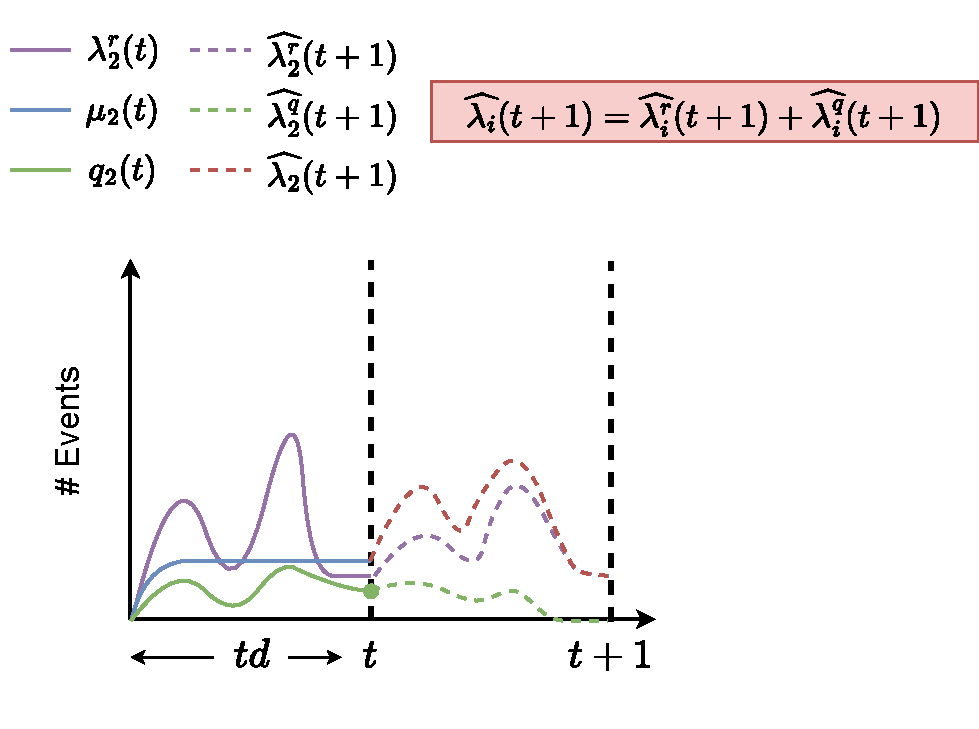
\includegraphics[scale=0.63]{images/concepts/predictive/PA-SPS-Prediction-14.pdf}
\end{figure}
\end{frame}

\begin{frame}{Predictive Approach : PA-SPS}
	\textbf{Prediction of number of active replicas}

	\begin{align*}
		r_i(t+1) = \frac{\widehat{\lambda_i}(t+1) \times et_i}{td}
	\end{align*}
	
%	\begin{tabular}{r l}
%	$r_i(t+1)$ & number of active replicas of operator $Oi$ computed at\\
%			   & the end of $t$\\
%   	$\widehat{\lambda_i}(t+1)$ & predicted number of events to process by operator $O_i$\\
%   	 						   & during $t$ \\
%   	${et}_i$ & average execution time of one event by operator $O_i$ \\
%	$td$ & time interval duration \\
%   	\end{tabular}
\end{frame}

\begin{frame}{PA-SPS : Prediction of active replicas}
	\textbf{Planning algorithm}
	\begin{center}
	\begin{align*}
		r_i(t+1) = \frac{\widehat{\lambda_i}(t+1) \times et_i}{td}
	\end{align*}

    \begin{figure}
    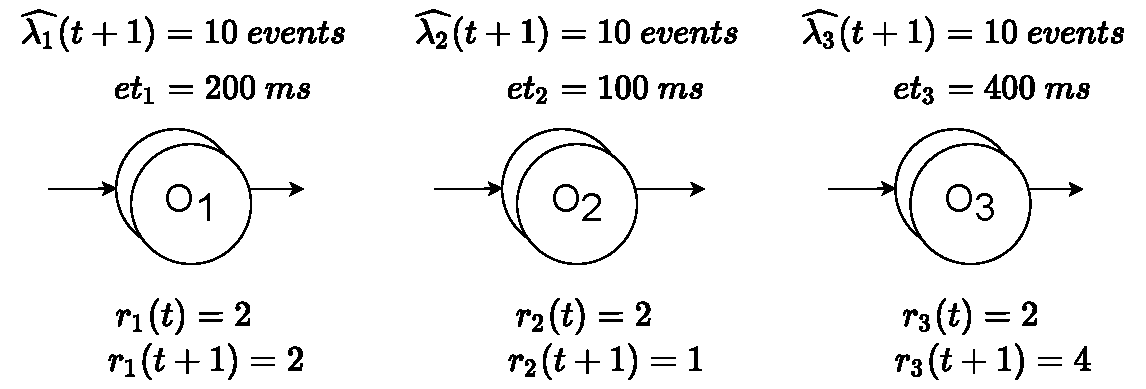
\includegraphics[scale=0.5]{images/concepts/predictive/PA-SPS-PredictiveModel.pdf}
    \end{figure}

    $td = 1000 ms$
   	\end{center}
\end{frame}